「swhandan.hsp」は、センサーボード上のスイッチを押すとメッセージが変わるかんたんなスクリプトです。早速、[F5]キーを押して実行してみましょう。


\begin{figure}[H]
    \begin{center}
      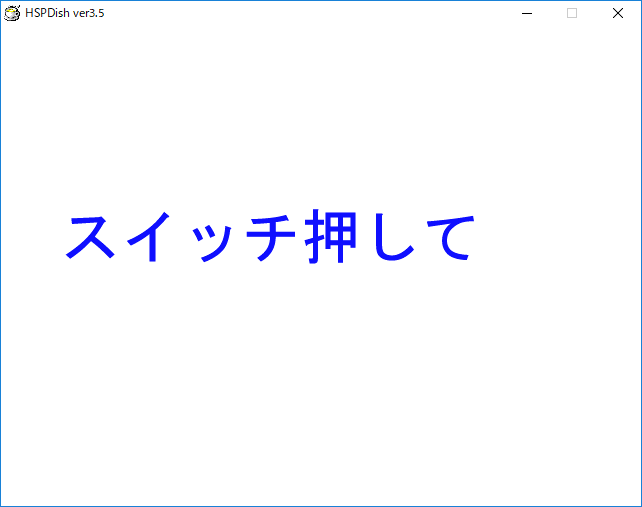
\includegraphics[width=7.673cm,height=6.05cm]{text04-img/text04-img003.png}
      \caption{swhandan.hspの実行画面}
    \end{center}
    \label{fig:read_from_directory}
\end{figure}


プログラムは最初の行から、下に向かって順番に実行されます。実際には、一瞬で過ぎてしまうのでわかりにくいですが、どのような順番でコンピューターが動くのか、想像しながら見てみることが大切です。わからない命令は以前の講座を復習してみましょう。

「*hata」から「goto *hata」までの間が「スイッチ押して」という文字を表示する部分です。





{\bfseries
*hata}

{\bfseries
\ \ redraw 0}

{\bfseries
\ \ font {\textquotedbl}{\textquotedbl},60}

{\bfseries
\ \ pos 60,180}

{\bfseries
\ \ color 0,0,255}

{\bfseries
\ \ mes {\textquotedbl}スイッチ押して{\textquotedbl}}

{\bfseries
\ \ redraw 1}

{\bfseries
\ \ await 16}

{\bfseries
\ \ if gpioin(5)=0 : goto *hata2}

{\bfseries
\ \ goto *hata}


ここでセンサーボードのスイッチを押すと流れが変わります。

{\bfseries
*hata2}

{\bfseries
\ \ redraw 0}

{\bfseries
\ \ font {\textquotedbl}{\textquotedbl},60}

{\bfseries
\ \ pos 60,180}

{\bfseries
\ \ color 255,0,0}

{\bfseries
\ \ mes {\textquotedbl}押しましたね!{\textquotedbl}}

{\bfseries
\ \ redraw 1}

{\bfseries
\ \ await 16}

{\bfseries
\ \ if gpioin(6)=0 : goto *hata}

{\bfseries
\ \ goto *hata2}


